\documentclass{article}
\usepackage{amsmath}
\usepackage[pdftex]{graphicx}
\usepackage{hyperref}

\begin{document}
\author{Tobias Reisch}
\title{Report on readAFM}
\maketitle

\section{The Project}

The goal of this project was to explore the possibilities of using Machine Learning to analyze data obtained from Non Contact Atomic Force Microscopy (NC-AFM). In particular functionalized tip NC-AFM, which allows to achieve atomic resolution \cite{gross2009chemical}.

This report contains a brief description of the most important steps in the project, especially
\begin{itemize}
\item How to generate the input data.
\item How to generate the labels.
\item How the Neural Net was built.
\item Highlights of the Results and an Outlook.
\end{itemize}

About the title: The git-repository was named \emph{readAFM} in intentional similarity to \emph{mechAFM}, while \emph{mechAFM} simulates an AFM image with a mechanical model of the tip atoms, \emph{readAFM} was the attempt to understand the output "images" of an AFM, in a sense "read" them.

The code written in the course of this internship is available under \\ \href{https://github.com/SINGROUP/readAFM/}{https://github.com/SINGROUP/readAFM/}.


\newpage
\section{Input}

Machine Learning usually needs a lot of training data to work. In our case this would be measured frequency shifts or forces from AFM experiments. Since there is no preexisting database of labeled experimental AFM 'images' available, we decided to use simulated data. We used the \emph{MechAFM} program, developed in our group, based on \cite{hapala2014, hamalainen2014}, to generate three dimensional arrays filled with force values. The inputs for \emph{MechAFM} consist of a xyz-file, a file specifying the potentials to use for the molecular dynamics simulation and a set of parameters. The values used that deviate from the default parameters are:

\begin{center}
\begin{tabular}{|c|c|}
\hline area & 8 {\AA} x 8 {\AA} \\ 
\hline zlow & position of topmost atom + 4 {\AA} \\ 
\hline zhigh & zlow + 4 {\AA} \\ 
\hline dx,dy,dz & 0.2 {\AA} \\ 
\hline 
\end{tabular} 
\end{center}

The output of \emph{MechAFM} consists of the force acting on the tip in z-direction, the angle of the CO-molecule and the displacement of the tip atom. We only keep the force in z-direction, which is compiled to a \emph{Numpy} array and stored in a hdf5-container. Additionally we store informations like the name string, the position of the atoms, the array-size, etc. as attributes in the hdf5-file. The data is separated randomly into a training and a validation set, with roughly a 80:20 splitting.

% Maybe mention the structure of the hdf5 files?

\newpage

\section{Labels}
For this large amount of simulated AFM data, we need to generate labels automatically. This step should be done very carefully, because the labels will also determine what the output of the Neural Net will look like. If we assign labels containing more information about the molecule than there is in the AFM data, the NN will not be able to train successfully, on the other hand, we want to get as much out of it as possible. We could, of course, ask the NN to predict the chemical sum formula for the molecule, but for this sort of analysis, there are already many different techniques available. And it is the big strength of atomic resolution AFM, that it is able to determine the spatial structure of the molecules. So the labels are a balance between extracting as much information as possible, determining the spatial structure of the molecule and bringing it into a form that is useful for the NN to learn. For example it is easier to ask for a constant length output, than for a variable length output (i.e. the NN outputs a list of atom positions).

For our case we decided it would be best (at the beginning) to produce a xy-map with values that are large when there is an atom at that position and zero otherwise. It is to a probability map of finding an atom at that position, but due to its lack of normalization it certainly is not. Therefor let's call it \emph{signal}.  A projection of the atoms coordinates to the xy-plane, but replacing the atoms with Gaussians scaled according to the covalent radius of the element. The formula for the Gaussians looks like this:

\begin{equation}
amp(element) = amp_0 * \frac{covalent radius(element)}{covalent radius(carbon)}
\end{equation}
\begin{equation}
\sigma = \sigma_0 * \frac{covalent radius(element)}{covalent radius(carbon)}
\end{equation}
\begin{equation}
signal(\vec{r}) = amplification*\exp(-\frac{(\vec{r}-\vec{r_0})^2}{\sigma^2})
\end{equation}

Where $amp_0$ and $\sigma_0$ are the input parameters and $\vec{r_0}$ is the position of the atom. To take into account, that atoms that are further away from the tip than others are less visible, we interpret the Gaussians as Gaussians in three dimensions and evaluate them at every point in the xy-plane at the height (z-value) of the topmost atom. It turned out to be beneficial to use different values for $\sigma$ in the xy-plane and in the z-direction. See also fig \ref{fig:gaussians}.

 \begin{figure}[htbp]
 	\begin{center}
 		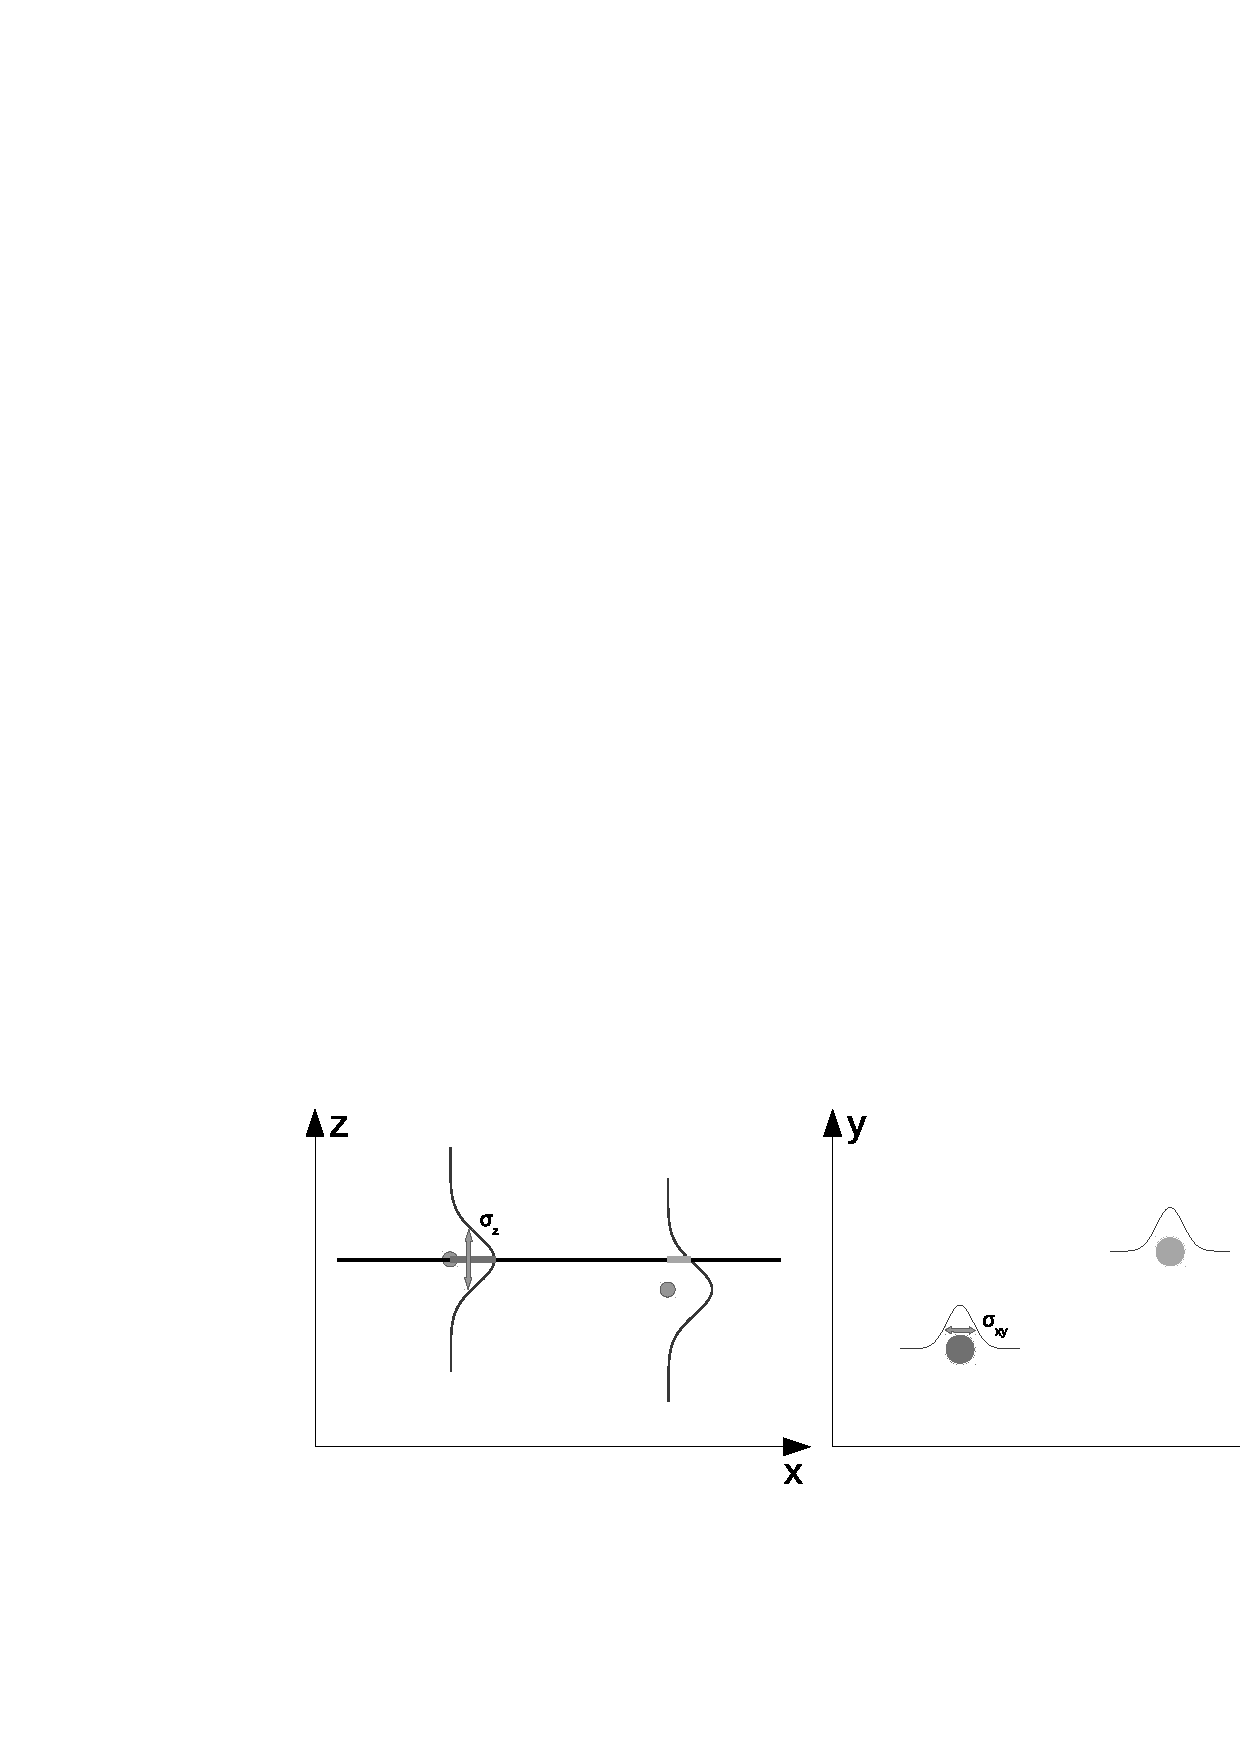
\includegraphics[width=9cm]{figs/gaussians.png}
 		\caption{Schematic explanation of the labelling process. The atoms with a large \emph{signal}-value at the height of the topmost atom (left image) appear brighter (darker red) in the projection to the xy-plane (left image).}
 		\label{fig:gaussians}
 	\end{center}
 \end{figure}

It is crucial to choose $\sigma_z$ carefully, since for a to large value all the atoms would appear in the labels whereas the atoms far away from the tip would not appear in the force images, on the other hand for a too small $\sigma_z$ only the topmost atom would be included in the labels, while in the force curves also lower lying atoms appear.

To determine $sigma_z$ rigorously we used a concept known from Information Theory, Mutual Information, which has recently been introduced to our group \cite{MIestimator}. The idea is that Mutual Information is large when two distributions contain similar information and small else. We calculated MI vs. $\sigma_z$ curves \ref{fig:MIcurve}, and they show a clear maximum.

 \begin{figure}[htbp]
 	\begin{center}
 		\includegraphics[width=10cm]{figs/Mutual_information-fullDB-k5_amp10_n1000.png}
 		\caption{Mutual Information vs. $\sigma_z$ for three dimensional molecules in random orientations. The spread can be explained by the fact, that the 1000 samples to calculate MI at every point were drawn randomly every time.}
 		\label{fig:MIcurve}
 	\end{center}
 \end{figure}



\newpage
\section{CNN}
In recent years there have been great advances with deep learning and Convolutional Neural Nets \cite{krizhevsky2012imagenet} and using them for automated analysis of experiments \cite{kraus2017automated}. We try to apply this technique in our case to analyze AFM data. For our task using a CNN seems feasible, for several reasons:
\begin{itemize}
\item Its translational invariance allows to use the same filters for different sized images of the same resolution.
\item The use of filters of a particular size can account for the flexibility of the CO-molecule at the end of the tip.
\end{itemize}

 \begin{figure}[htbp]
 	\begin{center}
 		\includegraphics[width=12cm]{figs/minimal_CNN.png}
 		\caption{Schematic representation of our NN, see explanation in the running text.}
 		\label{fig:NNstruct}
 	\end{center}
 \end{figure}

Our dataset can be imagined as a tensor of order 4, three indices for the spatial degrees of freedom (x,y,z) and one index for the "input channels", when treating color images this number is three, for the three color channels RGB. In our case there is just one input channel, the forces. In the first convolutional layer, this tensor is convolved with 16 filters of the size 0.8 x 0.8 x 0.8{\AA}, the convolution preserves the spatial size of the tensor, but the number of "channels" grows to 16. After applying the hyperbolic tangent function as nonlinearity, we repeat the convolution step with 32 filters.

After the 3D convolutions preserved the order of the tensor, now we want to reduce it to a two dimensional image. To achieve this, we flatten the axes of the tensor corresponding to z and the channels and use them as input to a fully connected layer. After the fully connected layer we apply a rectified linear (ReLU) operation as nonlinearity and we receive the output. To stay with the language of tensors: Now we have a tensor of order three, two spatial degrees of freedom and one output channel. The size of the spatial axes is conserved. For a schematic explanation see fig. \ref{fig:NNstruct}.

For this Neural Net the filters of the convolution and the weights and biases can be trained with gradient descent. We used stochastic training with the Adam Optimizer \cite{kingma2014adam}, which was especially designed for this purpose. 

To use gradient descent we need to determine a scalar value as "cost" function which can then be minimized. We start out calculating a value for the "accuracy" which is the summed squared difference between the prediction of the NN and the label.

\begin{equation}
accuracy = \sum_{x, y} (v_{pred}(x,y)-v_{sol}(x,y))^2
\end{equation}

Where v(x,y) should represent the greyscale value at the position (x,y). This measure works to train the NN and is a good characteristic for the convergence of a training session. However, for small $\sigma_{xy}$ and small $amp$, the gradient descent would train the weights and biases to a state where they would just output zero everywhere. To prevent this, we adapted the accuracy function by multiplying it at each position (pixel) with the solution, see Eqn. \eqref{eq:acc_weighted}. Because $v_{sol}$ is 0 everywhere except at the positions of the atoms, this represents an extra penalty for false negatives (showing no atom even when there should be one). The $\frac{1}{amp}$ compensates for the fact that $v_{sol}$ ranges between 0 and amp, not 0 and 1.

\begin{equation}
accuracy_{weighted} = \sum_{x, y} \frac{1}{amp}* v_{sol}(x,y)*(v_{pred}(x,y)-v_{sol}(x,y))^2
\label{eq:acc_weighted}
\end{equation}

If only the weighted accuracy is used, there is no penalty to false positives (showing atoms where none should be) anymore. To prevent this, the cost function is made up by a mix of both accuracies, the proportionality can be determined by a parameter c (costWeight in the \emph{parameters.in} file).

\begin{equation}
cost = c*accuracy + (1-c)*accuracy_{weighted}
\end{equation}

The accuracy and trainability of this Neural Net can be changed in a several ways: By changing the filter size and number in the convolutions, using different sized fully connected layers (a FC layer with 64 neurons already works, but using larger FC layers improves the result drastically!) and of course adding more layers. The effect of these changes will be discussed in the next section.


\newpage
\section{Results}

Although the goal of the project is clearly set to use ML to understand better AFM images of arbitrary molecules, it was more practical to start with a simplified task. At first we had a database filled with single atoms at random positions, mainly to debug and as a sanity check. Then we followed the "historical" route and produced a database of flat molecules (where the heavy atoms (everything except H) are all in one plane). The first functionalized tip NC-AFM experiments with atomic resolution were also performed on flat molecules, because a corrugation in z complicates the task even more. Which is what we did in a third step. We used 1000 molecules from \cite{ramakrishnan2014quantum} and simulated each in 100 random orientations.

The analysis for the flatDB worked quite well. Our CNN was able to predict the correct positions of the atoms quite well, or a few examples see figure \ref{fig:resultsflatDB}. It became apparent that especially a larger hidden layer improves the performance a lot. 

\begin{figure}[htbp]
	\begin{center}
		\includegraphics[width=14cm]{figs/flatMolecules_HL512/collection.png}

		\caption{Flat molecules analyzed with the NN configuration: Conv3D 4x4x4x16, Conv3D 4x4x4x32, FC512}
		\label{fig:resultsflatDB}
	\end{center}
\end{figure}

For the database filled with random three dimensional molecules in random orientations there is the extra problem, that not all parts of the molecule are visible. To find the optimal $\sigma_z$ we tried to maximize the Mutual Information for the $F_z$-tensor and the solution-"image" as a function of $\sigma_z$, this value agreed quite well with the previous estimate (just from looking at it). However, the resulting predictions are not as good as they are for the flat molecules. In figure \ref{fig:resultsfullDB} the results of the  most basic configuration are shown, the positions of the atoms are not predicted as well as for the flat molecules. We were also not able to improve them much with bigger hidden layers.

\begin{figure}[htbp]
	\begin{center}
		\includegraphics[width=14cm]{figs/fullDB_base/collection.png}
		\caption{Random molecules analyzed with the NN configuration: Conv3D 4x4x4x16, Conv3D 4x4x4x32, FC64}
		\label{fig:resultsfullDB}
	\end{center}
\end{figure}

Here is a table of configurations that were tried:

\begin{center}
\begin{tabular}{|l|}
\hline conv3d(4x4x4x16) tanh conv3d(4x4x4x32) tanh hl64 relu \\
\hline conv3d(4x4x4x16) tanh conv3d(4x4x4x32) tanh hl128 relu \\
\hline conv3d(4x4x4x16) tanh conv3d(4x4x4x32) tanh hl256 relu \\
\hline conv3d(4x4x4x16) tanh conv3d(4x4x4x32) tanh hl512 relu \\
\hline conv3d(4x4x4x16) tanh conv3d(4x4x4x32) tanh hl1024 relu \\
\hline conv3d(8x8x8x16) tanh conv3d(8x8x8x32) tanh hl64 relu \\
\hline conv3d(8x8x8x16) tanh conv3d(8x8x8x32) tanh hl256 relu \\
\hline conv3d(4x4x4x16) tanh conv3d(4x4x4x32) tanh hl64 relu conv2d(4x4x16) relu \\
\hline conv3d(4x4x4x16) tanh conv3d(4x4x4x32) tanh conv2d(4x4x32) tanh hl64 relu \\
\hline
\end{tabular}
\end{center}

We also tested for which $\sigma_{xy}$/amp combinations successful training was possible and when it would just converge to 0 everywhere, we were able to prove that the improved cost function made the values for $\sigma_xy$/amp much lower. It is also possible to avoid local minimal by starting from a larger $\sigma_{xy}$ and use that weights and biases as a starting point to train for smaller $\sigma_{xy}$.

\newpage
\section{Outlook}

Possibly adding an extra convolutional layer or more hidden layers could improve the results. An option also worth considering might be to apply extra operations on the output layer. These could either be some filters, e.g. a search for local maxima, or again a Neural Net, e.g. convolutional layer that is trained separately from the CNN.

Maybe the cut through the Gaussians at the height of the topmost atom, is not optimal. From a physical perspective doing the cut at the lowest position of the tip could also make sense.

We already contacted experimentalists, about NC-AFM data which we could use our NN on. Potential insights include whether the training on data simulated with \emph{MechAFM} works, or if a more sophisticated model is necessary. It would also test our model for its robustness against experimental artifacts.

The exchange with experimentalists is also very valuable with regard to the future direction of this project: What form of possible applications for automated (NC-)AFM experiments would be the most welcome?




\newpage
\bibliographystyle{unsrt}
\bibliography{readAFM}

\end{document}



